For each model we used state polls which only include Biden and Trump as candidates, taken between May 03, 2020 and October 31, 2020 aggregated by \cite{fivethirtyeight}.
\\~\\
We evaluate each model using a mean absolute error (MAE) over states, as shown in table \ref{tab:all_models_final_mae}, which can be interpreted as the vote share error for both candidates, since making a 3\% error in favor of Biden is equivalent to making a 3\% error against Trump. 
\begin{table}[H]
\centering
\caption{Final Results Mean Absolute Error}
\begin{tabular}{lrr}
\toprule
      model &  battleground MAE &  non-battleground MAE \\
\midrule
 ewma\_03\_lw &          0.019547 &              0.034726 \\
    ewma\_03 &          0.016324 &              {\bf 0.033381} \\
 ewma\_01\_lw &          0.023007 &              0.040461 \\
    ewma\_01 &          0.020694 &              0.036239 \\
     ewma\_1 &          {\bf 0.013867} &              0.035453 \\
\bottomrule
\end{tabular}
    \label{tab:all_models_final_mae}
\end{table}

In table \ref{tab:all_models_final_mae}, we can see that every model performs substantially better on battleground states than on non-battleground states, supporting our primary hypothesis, that battleground states will actually be more predictable than non-battleground states.
\\~\\
Interestingly, the sample size weighted models performs worse for each model compared to their unweighted versions. We hypothesized that battleground states may perform better due to more frequent polling; about twice as many polls are conducted in battleground states compared to non-battleground states, shown in Figure \ref{fig:aggregate_polling_2020-05-01_-_2020-10-31_number_of_polls}. However, despite polling more frequently, the sample size tends to be slightly smaller for battleground states in table \ref{tab:aggregate_polling_2020-05-01_-_2020-10-31_mean_sample_size}. So it may be the case that discounting polls with smaller sample sizes, might slightly negate the benefit of having more polls in battleground states. 

\begin{table}[H]
    \centering
    \begin{table}
\centering
\caption{Aggregate Polling (2020-05-01 - 2020-10-31) Mean Sample Size}
\label{table:aggregate\_polling\_2020-05-01\_-\_2020-10-31\_mean\_sample\_size}
\begin{tabular}{lr}
\toprule
 battleground &  samples mean \\
\midrule
        False &   2835.778209 \\
         True &   2659.970856 \\
\bottomrule
\end{tabular}
\end{table}

    \label{tab:aggregate_polling_2020-05-01_-_2020-10-31_mean_sample_size}
\end{table}

\subsection{Bias and Predictability}
Polling methodology varies from pollster to pollster, but demographic stratification weighting is commonly used for general election polling in the US and elsewhere, as described in \cite{Lauderdale2020ModelbasedPP}. While it may be difficult to determine whether a pollster has chosen the right post stratification weights, we can consider the effects of polls altogether to determine whether they consistently make mistakes in the same direction. 

\begin{figure}[H]
    \centering
    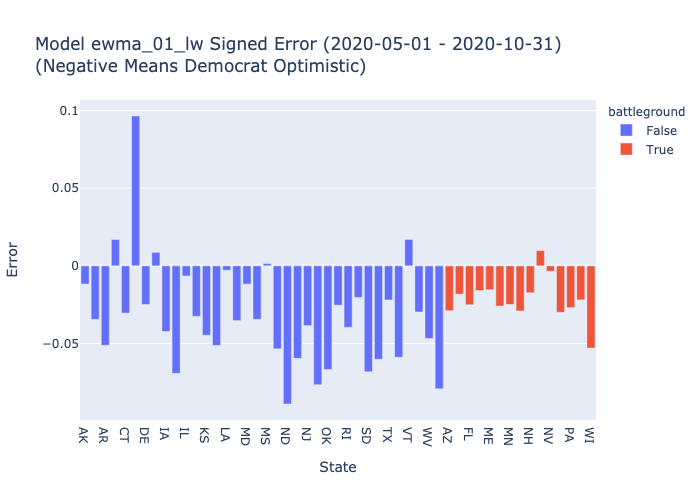
\includegraphics[height=25em]{figures/ewma_01_lw_2020-05-01-2020-10-31_signed_error.png}
    \label{fig:ewma_01_lw_2020-05-01-2020-10-31_signed_error}
\end{figure}


\begin{figure}[H]
    \centering
    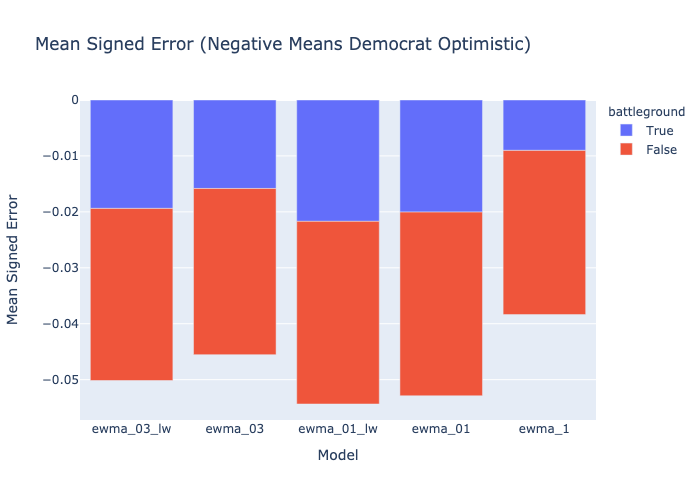
\includegraphics[height=26em]{figures/ewma_03_lw_ewma_03_ewma_01_lw_ewma_01_ewma_1_mean_signed_error.png}
    \label{fig:ewma_03_lw_ewma_03_ewma_01_lw_ewma_01_ewma_1_mean_signed_error}
\end{figure}
